\section{Not\_\-Predicate$<$ Predicate\-Neg $>$ Class Template Reference}
\label{class_not___predicate}\index{Not_Predicate@{Not\_\-Predicate}}
{\bf Predicate}{\rm (p.\,\pageref{class_predicate})} that return the negation of a predicate passed in parameter.  


{\tt \#include $<$Not\_\-Predicate.hxx$>$}

Inheritance diagram for Not\_\-Predicate$<$ Predicate\-Neg $>$::\begin{figure}[H]
\begin{center}
\leavevmode
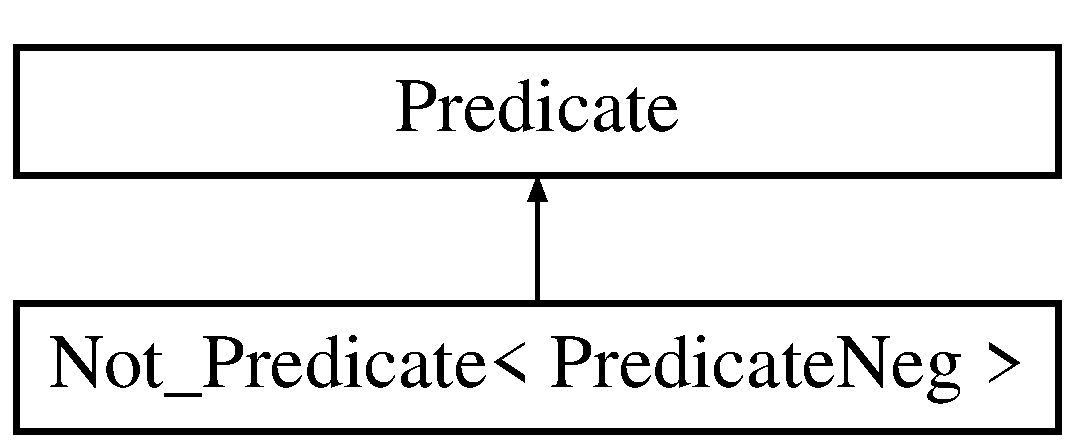
\includegraphics[height=2cm]{class_not___predicate}
\end{center}
\end{figure}
\subsection*{Public Member Functions}
\begin{CompactItemize}
\item 
{\bf Not\_\-Predicate} (Predicate\-Neg \&in\-Pred)\label{class_not___predicate_48a08a2ead6b824a9fec80c3610ccba7}

\begin{CompactList}\small\item\em Constructor. \item\end{CompactList}\item 
template$<$class Iterator, class Measure$>$ bool {\bf operator()} (Iterator it\-Cand, Measure \&mes\-Cand)\label{class_not___predicate_c4dd938a356c8476e50806158069d169}

\begin{CompactList}\small\item\em Operator that test if a set of attributes is not redundant. \item\end{CompactList}\item 
template$<$class Cand\_\-Data\-Struct, class f$>$ void {\bf pre\-Processing} (Cand\_\-Data\-Struct \&cand, f \&word\-To\-Set)
\begin{CompactList}\small\item\em Function used to do some pre processing operations before testing the candidates generated. \item\end{CompactList}\item 
template$<$class Cand\_\-Data\-Struct, class f$>$ void {\bf post\-Processing} (Cand\_\-Data\-Struct \&cand, f \&word\-To\-Set)
\begin{CompactList}\small\item\em Function used to do some post processing operations after testing the candidates generated. \item\end{CompactList}\end{CompactItemize}
\subsection*{Protected Attributes}
\begin{CompactItemize}
\item 
Predicate\-Neg $\ast$ {\bf pred}\label{class_not___predicate_2dff4f17e32eeae61ee949f76e542ff5}

\begin{CompactList}\small\item\em {\bf Predicate}{\rm (p.\,\pageref{class_predicate})} to studied. \item\end{CompactList}\end{CompactItemize}


\subsection{Detailed Description}
\subsubsection*{template$<$class Predicate\-Neg$>$ class Not\_\-Predicate$<$ Predicate\-Neg $>$}

{\bf Predicate}{\rm (p.\,\pageref{class_predicate})} that return the negation of a predicate passed in parameter. 



\subsection{Member Function Documentation}
\index{Not_Predicate@{Not\_\-Predicate}!postProcessing@{postProcessing}}
\index{postProcessing@{postProcessing}!Not_Predicate@{Not\_\-Predicate}}
\subsubsection{\setlength{\rightskip}{0pt plus 5cm}template$<$class Predicate\-Neg$>$ template$<$class Cand\_\-Data\-Struct, class f$>$ void {\bf Not\_\-Predicate}$<$ Predicate\-Neg $>$::post\-Processing (Cand\_\-Data\-Struct \& {\em cand}, f \& {\em word\-To\-Set})\hspace{0.3cm}{\tt  [inline]}}\label{class_not___predicate_849572f82b1b8a34b9b71459c9da24be}


Function used to do some post processing operations after testing the candidates generated. 

\begin{Desc}
\item[Parameters:]
\begin{description}
\item[{\em cand}]container of words of the language. \end{description}
\end{Desc}
\index{Not_Predicate@{Not\_\-Predicate}!preProcessing@{preProcessing}}
\index{preProcessing@{preProcessing}!Not_Predicate@{Not\_\-Predicate}}
\subsubsection{\setlength{\rightskip}{0pt plus 5cm}template$<$class Predicate\-Neg$>$ template$<$class Cand\_\-Data\-Struct, class f$>$ void {\bf Not\_\-Predicate}$<$ Predicate\-Neg $>$::pre\-Processing (Cand\_\-Data\-Struct \& {\em cand}, f \& {\em word\-To\-Set})\hspace{0.3cm}{\tt  [inline]}}\label{class_not___predicate_8282dfa9cdd77232c633264d73cab680}


Function used to do some pre processing operations before testing the candidates generated. 

\begin{Desc}
\item[Parameters:]
\begin{description}
\item[{\em cand}]container of words of the language. \end{description}
\end{Desc}


The documentation for this class was generated from the following file:\begin{CompactItemize}
\item 
F:/i\-Zi/algorithms/Not\_\-Predicate.hxx\end{CompactItemize}
